\section{\gls{DPR} for Internal Fault Mitigation}\label{InternalFaults}
\begin{figure}
    \centering
    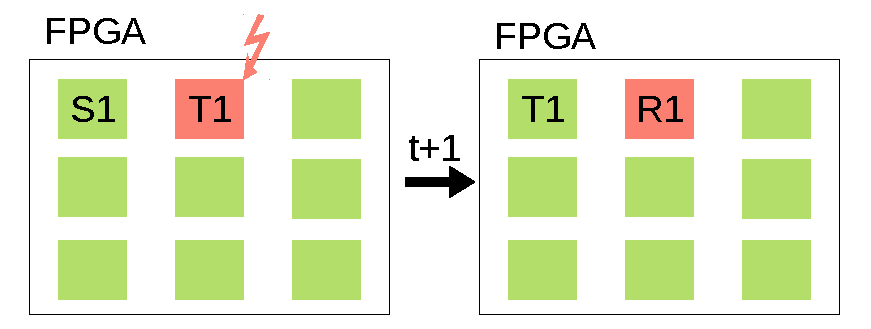
\includegraphics[width=\columnwidth]{graphics/faultyTile2.pdf}
    %\resizebox{\smallColumnWidth}{!}{\tikzset{every picture/.style={line width=0.25pt}} %set default line width to 0.75pt        

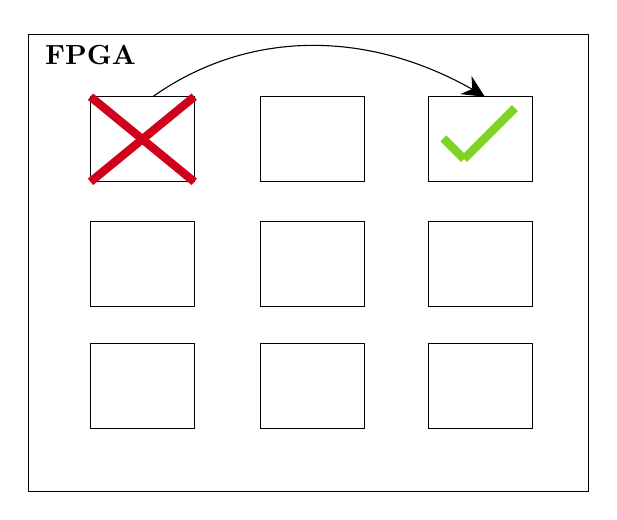
\begin{tikzpicture}[x=0.75pt,y=0.75pt,yscale=-1,xscale=1]
%uncomment if require: \path (0,279); %set diagram left start at 0, and has height of 279

%Shape: Rectangle [id:dp5787797491333819] 
\draw   (6,20) -- (276,20) -- (276,240) -- (6,240) -- cycle ;
%Shape: Rectangle [id:dp17505095690594463] 
\draw   (36,50) -- (86,50) -- (86,91) -- (36,91) -- cycle ;
%Shape: Rectangle [id:dp3058047377979807] 
\draw   (36,110) -- (86,110) -- (86,151) -- (36,151) -- cycle ;
%Shape: Rectangle [id:dp004684645465554249] 
\draw   (36,169) -- (86,169) -- (86,210) -- (36,210) -- cycle ;
%Shape: Rectangle [id:dp3077757040785931] 
\draw   (118,50) -- (168,50) -- (168,91) -- (118,91) -- cycle ;
%Shape: Rectangle [id:dp7450799349257811] 
\draw   (118,110) -- (168,110) -- (168,151) -- (118,151) -- cycle ;
%Shape: Rectangle [id:dp2725857150503048] 
\draw   (118,169) -- (168,169) -- (168,210) -- (118,210) -- cycle ;
%Shape: Rectangle [id:dp3816815123242099] 
\draw   (199,50) -- (249,50) -- (249,91) -- (199,91) -- cycle ;
%Shape: Rectangle [id:dp2885393682660524] 
\draw   (199,110) -- (249,110) -- (249,151) -- (199,151) -- cycle ;
%Shape: Rectangle [id:dp4969175268738504] 
\draw   (199,169) -- (249,169) -- (249,210) -- (199,210) -- cycle ;
%Straight Lines [id:da8580754234796655] 
\draw [color={rgb, 255:red, 208; green, 2; blue, 27 }  ,draw opacity=1 ][line width=3]    (36,50) -- (86,91) ;


%Straight Lines [id:da5772916268060835] 
\draw [color={rgb, 255:red, 208; green, 2; blue, 27 }  ,draw opacity=1 ][line width=3]    (86,50) -- (36,91) ;


%Curve Lines [id:da5702734861080319] 
\draw    (66,50) .. controls (112.04,17.33) and (171.3,17) .. (224.39,49.02) ;
\draw [shift={(226,50)}, rotate = 211.67000000000002] [fill={rgb, 255:red, 0; green, 0; blue, 0 }  ][line width=0.75]  [draw opacity=0] (10.72,-5.15) -- (0,0) -- (10.72,5.15) -- (7.12,0) -- cycle    ;

%Straight Lines [id:da7282259837027933] 
\draw [color={rgb, 255:red, 126; green, 211; blue, 33 }  ,draw opacity=1 ][line width=3]    (240.5,55.5) -- (216,80) ;


%Straight Lines [id:da7142424530641487] 
\draw [color={rgb, 255:red, 126; green, 211; blue, 33 }  ,draw opacity=1 ][line width=3]    (216,80) -- (206,70) ;



% Text Node
\draw (36,30) node  [align=left] {\textbf{FPGA}};


\end{tikzpicture}
}
    \caption{Internal Fault Mitigation - functionality from a faulty tile is moved to a healthy area with \gls{DPR}}\label{fig:internalFaultMitigation}
\end{figure}

%\tikzset{every picture/.style={line width=0.25pt}} %set default line width to 0.75pt        

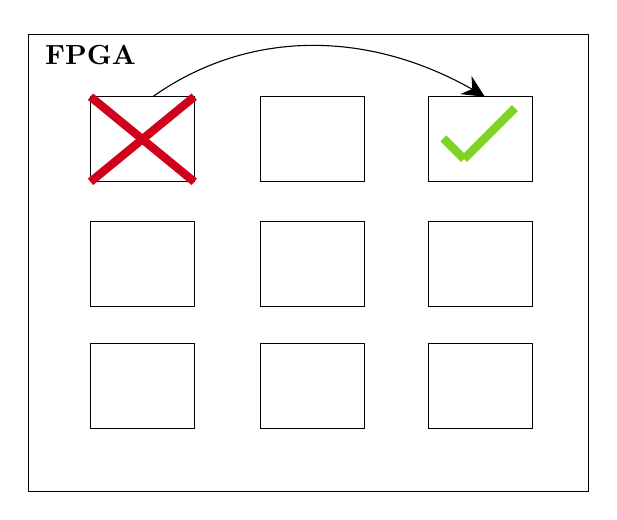
\begin{tikzpicture}[x=0.75pt,y=0.75pt,yscale=-1,xscale=1]
%uncomment if require: \path (0,279); %set diagram left start at 0, and has height of 279

%Shape: Rectangle [id:dp5787797491333819] 
\draw   (6,20) -- (276,20) -- (276,240) -- (6,240) -- cycle ;
%Shape: Rectangle [id:dp17505095690594463] 
\draw   (36,50) -- (86,50) -- (86,91) -- (36,91) -- cycle ;
%Shape: Rectangle [id:dp3058047377979807] 
\draw   (36,110) -- (86,110) -- (86,151) -- (36,151) -- cycle ;
%Shape: Rectangle [id:dp004684645465554249] 
\draw   (36,169) -- (86,169) -- (86,210) -- (36,210) -- cycle ;
%Shape: Rectangle [id:dp3077757040785931] 
\draw   (118,50) -- (168,50) -- (168,91) -- (118,91) -- cycle ;
%Shape: Rectangle [id:dp7450799349257811] 
\draw   (118,110) -- (168,110) -- (168,151) -- (118,151) -- cycle ;
%Shape: Rectangle [id:dp2725857150503048] 
\draw   (118,169) -- (168,169) -- (168,210) -- (118,210) -- cycle ;
%Shape: Rectangle [id:dp3816815123242099] 
\draw   (199,50) -- (249,50) -- (249,91) -- (199,91) -- cycle ;
%Shape: Rectangle [id:dp2885393682660524] 
\draw   (199,110) -- (249,110) -- (249,151) -- (199,151) -- cycle ;
%Shape: Rectangle [id:dp4969175268738504] 
\draw   (199,169) -- (249,169) -- (249,210) -- (199,210) -- cycle ;
%Straight Lines [id:da8580754234796655] 
\draw [color={rgb, 255:red, 208; green, 2; blue, 27 }  ,draw opacity=1 ][line width=3]    (36,50) -- (86,91) ;


%Straight Lines [id:da5772916268060835] 
\draw [color={rgb, 255:red, 208; green, 2; blue, 27 }  ,draw opacity=1 ][line width=3]    (86,50) -- (36,91) ;


%Curve Lines [id:da5702734861080319] 
\draw    (66,50) .. controls (112.04,17.33) and (171.3,17) .. (224.39,49.02) ;
\draw [shift={(226,50)}, rotate = 211.67000000000002] [fill={rgb, 255:red, 0; green, 0; blue, 0 }  ][line width=0.75]  [draw opacity=0] (10.72,-5.15) -- (0,0) -- (10.72,5.15) -- (7.12,0) -- cycle    ;

%Straight Lines [id:da7282259837027933] 
\draw [color={rgb, 255:red, 126; green, 211; blue, 33 }  ,draw opacity=1 ][line width=3]    (240.5,55.5) -- (216,80) ;


%Straight Lines [id:da7142424530641487] 
\draw [color={rgb, 255:red, 126; green, 211; blue, 33 }  ,draw opacity=1 ][line width=3]    (216,80) -- (206,70) ;



% Text Node
\draw (36,30) node  [align=left] {\textbf{FPGA}};


\end{tikzpicture}

\glspl{FPGA} provide high flexibility and good performance in many areas that require a high amount of concurrent computing and therefore benefit from a dedicated hardware implementation.
These properties prove useful for applications in the domain of aerospace and help to reduce the cost for satellites and spacecraft while providing high flexibility throughout the development process. 

But \glspl{FPGA} are especially vulnerable to cosmic radiation which can create a multitude of internal errors in the \gls{FPGA} and thereby breaking its intended functionality \cite{ito_total_2015}.
While there are radiation hardened \glspl{FPGA} available on the market, the mass of a space embedded system is still composed of 80\% radiation shielding \cite{ito_total_2015}.
Yet, this shielding is still not able to provide sufficient protection from radiation induced errors, especially on long term missions. 
Therefore, solutions for fault mitigation in aerospace \glspl{FPGA} need to be developed on the architectural level instead of the physical level. 
This may also provide the advantage of lower requirements for radiation shielding and therefore a reduced cost for payload on rocket launches.
Figure \ref{fig:internalFaultMitigation} depicts the basic concept of internal fault mitigation. 
An error occurs in Task 1 (\textit{T1}) and a healthy Spare Tile (\textit{S1}) is available. 
\textit{T1} is then moved to \textit{S1} in a partial-reconfiguration step and is ready for regular operation after the reconfiguration time \textit{t+1}.
A recovery of the tile Recovery 1 (\textit{R1}) is attempted and if it fails, it is marked as faulty for future reconfiguration operations.

The next section reviews the different types of faults and categorizes them. 

\subsection{Types of Internal Faults}
There are different types of faults that may occur in the lifetime of an \gls{FPGA}, a short overview over the most relevant ones is given in the following.
\par
\textbf{Transient Faults}
\begin{itemize}
    \item \glspl{SEU}, e.g. radiation induced \cite{alkady_fault-tolerant_2014}, \cite{lee_fault-tolerant_2017}
    \begin{itemize}
    \item Change of the logic state in a memory cell
    \item Commonly tackled by redundancy
    \item Built-in fault detection unit possible
    \end{itemize}
    \item Single Bit Errors (SBEs)
    \item Single Event Transients (SETs)
    \item Address Decoding Faults
\end{itemize}

Faults occur either in the interconnect of the \gls{FPGA} (which uses up to 80\% of the available silicon) or in its actual logic blocks \cite{alkady_fault-tolerant_2014}, \cite{jing_huang_routability_2004}.
\par
\textbf{Permanent Faults}
\begin{itemize}
    \item Time Dependant Dielectric Breakdowns (TDDBs)
    \item Electro Migration
    \item Hot Carrier Effect
\end{itemize}

Based on this review, two main categories of errors emerge.
Firstly, \textit{permanent faults} (also known as \textit{hard errors}), which include all faults that render the affected area completely unusable. 
Secondly, \textit{transient faults} (also known as \textit{soft errors}), which encompasses faults where a reclamation of the erroneous area may still be possible after the initial mitigation process.

To mitigate the aforementioned internal faults in an \gls{FPGA}, different strategies can be employed.
All of them feature \gls{DPR} as a means to move functional blocks from a faulty silicon area to a healthy one.
What sets them apart is the way of fault detection and the specifically employed \gls{DPR} strategy.

The following section introduces the general concept of a fault mitigation- and recovery flow. 

\subsection{Abstract Fault Mitigation Flow}\label{AbstractFaultMitigationFlow}
As the general scheme for fault mitigation is always the same, a brief introduction to the corner stones of every recovery flow is given (depicted in figure \ref{fig:internalFaultFlow}). 

\subsubsection{Detect Fault}
    One key aspect of fault mitigation is fault detection. 
    When faulty behaviour is detected, the origin of the fault needs to be determined.
    Generally, a dedicated (internal or external) control-unit is assigned to the task of result verification.
    This control-unit then gathers information about the location of the affected area and which functionality is corrupted.
\subsubsection{Mitigate Fault}
    After a successful isolation of the fault, steps towards its mitigation are taken.
    Due to external (e.g. increase in radiation) or internal (e.g. space, power) constraints, this stage may encompass some sort of estimation algorithm for the selection of a suitable \gls{PR} block.
    As a consequence, the system can dynamically adapt its fault resistance to changing circumstances.
\subsubsection{Resume Functionality}
    To fully leverage the advantage of \gls{DPR}, some sort of redundancy (e.g. \gls{TMR}) is usually employed.
    This allows the whole system to remain fully functional during the process of \gls{DPR} - the redundant modules will still provide the required data / processing during the reconfiguration. 
    The now freshly instantiated module then needs to re-sync its state with the rest of the system to return to its normal functionality.
\subsubsection{Recover Faulty Area}
    If a transient fault is responsible for the erroneous behaviour, the affected chip area may be recovered by error correction techniques like scrubbing \cite{reorda_error-detection_2017}. 
    In case of a successful recovery, the control-unit can mark the partition as healthy and reuse it at a later point in time.
\begin{center}
\begin{figure}[h]
    \centering
    \resizebox{\smallColumnWidth}{!} {
            \definecolor{one}{HTML}{E52B50}
    %\definecolor{two}{HTML}{fb8072}
    \definecolor{two}{HTML}{80b1d3}
\begin{tikzpicture}[]

\draw[solid]
(-2,0) node[fill=one!20,draw,rounded corners] (B) {Detect Fault}
(1,-1) node[fill=two!20,draw] (C) {Locate Affected Area}
(1,-2) node[fill=two!20,draw] (D) {Determine Affected Functionality}
(1,-3) node[fill=two!20,draw] (E) {Select Suitable PR Block}
(1,-4) node[fill=two!20,draw] (F) {Instantiate PR Block}
(1,-5) node[fill=one!20,draw] (G) {Resume Functionality}
(1,-6) node[fill=two!20,draw] (H) {Recover Faulty Area};
%\draw[dotted] (4, 2) -- (4,-3);
\draw[->, to path={-| (\tikztotarget)}] (B) edge (C);
\draw[->] (C) edge (D);
\draw[->] (D) edge (E);
\draw[->] (E) edge (F);
\draw[->] (F) edge (G);
\draw[->] (G) edge (H);
%\draw[->, to path={-| (\tikztotarget)}] (D) edge (E);
%\draw[->] (E) edge (F);
%\draw[->, to path={-| (\tikztotarget)}] (F) edge (G);
%\draw[->] (G) edge (H);
%\draw[->, to path={-| (\tikztotarget)}] (F) edge (G);
%\draw[->, to path={-| (\tikztotarget)}] (G) edge (H);
%\draw[->, to path={-| (\tikztotarget)}] (H) edge (A);
\draw[->, to path={-| (\tikztotarget)}] (G) edge (B);
\draw[->, to path={-| (\tikztotarget)}] (H) edge (B);
\end{tikzpicture}

    }
\caption{Abstract Fault Mitigation Flow}
\label{fig:internalFaultFlow}
\end{figure}
\end{center}
Each stage of this flow can be implemented with different architectural design choices.
These choices are influenced by available resources, real-time constraints and the desire of more control over the system behaviour.
The next sections introduce different architectures for a system that wants to utilize \gls{DPR} for fault mitigation.

\subsection{Spare Tile Architecture for \gls{DPR}}\label{sec:SpareTileArchitecture}
This approach is taken in the work of \cite{lameres_radsat_nodate} and is extended in \cite{wilson_hybrid_2017}.
It creates a computer system that exhibits a higher fault tolerance against radiation induced faults while using only commercially available off-the-shelf \glspl{FPGA}. 
To achieve this, the computing system is designed as a \gls{PR} partition from the beginning (figure \ref{fig:SpareTileArchitecture}). 
\gls{TMR} with a voter is used to assess the correctness of the output. 
When one module fails to compute the expected result (i.e. the result of the other two modules), a partial reconfiguration flow is triggered.
One of the healthy spare tiles is selected for the instantiation of another compute module.
The usage of the scrubbing technique allows the eventual recovery of the faulty tile which decreases the likelihood of resource exhaustion. 
Scrubbing is also used to check the health of inactive tiles in intervals, so that the healthiness of the backup tiles is known at all time. 
An advantage of this approach is that all relevant computations can still be carried out by the two remaining healthy modules during the recovery process. 
It also increases the robustness of the system in comparison to a stand-alone \gls{TMR} + scrubbing approach.
The system has been verified theoretically by a Markov model, as well as in a real world scenario where the test system was exposed to a defined dose of radiation over a time-period (The \gls{MTBF} was increased by a factor of 90 in this test).

A system like this is easy to implement and creates a low resource overhead during the development phase while it provides drastically improved reliability.
The verification of the results in the voter and the selection of a healthy healthy spare tile for reconfiguration don't pose a significant computational load on the system.
As instantiation of a spare module is way faster than scrubbing a faulty tile (1ms vs 100ms), the chance of losing 2 active compute tiles in a short time frame is reduced. 
But as the complexity of such a design increases, the tile size also increases. 
This implies an increased overall area cost for the spare tiles on the \gls{FPGA} which makes efficient placement more difficult.
It also reduces the amount of available space for other desired functionalities. 

The work of \cite{martins_tmr_2015} follows a similar principle, but tries to optimize the tooling that is required for partial bitstream generation.
The goal of these optimizations is to reduce the overall resource waste by the provision of only one partial bitstream per module for all \textit{N} \glspl{RP}. %The following part could still be extended with more details 
Usual \gls{DPR} workflows require a dedicated partial bitstream for each \gls{RP}, which results in \textit{N} partial bitstreams for \textit{N} desired \glspl{RP}.
\cite{martins_dynamic_2018} improves the previous work in \cite{martins_tmr_2015} and demonstrates its functionality in a scenario where permanent faults due to ageing are detected and mitigated.
\begin{center}
\begin{figure}[h]
    \centering
    \resizebox{\columnwidth}{!} {
        \begin{tikzpicture}[]

\draw[solid]

(0,2) node[fill=cBlue!40,draw, minimum height=1.5cm, minimum width=2.5cm] (ASV) {\textbf{Voter / Control}}
(-3,0) node[fill=cYellow!60,draw, minimum height=1.5cm, minimum width=2.5cm] (AS) {Compute Tile}
(0,0) node[fill=cYellow!60,draw, minimum height=1.5cm, minimum width=2.5cm] (AM) {Compute Tile}
(3,0) node[fill=cYellow!60,draw, minimum height=1.5cm, minimum width=2.5cm] (AE) {Compute Tile}
(-3,-2) node[fill=cGreen!60,draw, minimum height=1.5cm, minimum width=2.5cm] (ASS) {Spare Tile}
(0,-2) node[fill=cGreen!60,draw, minimum height=1.5cm, minimum width=2.5cm] (AMS) {Spare Tile}
(3,-2) node[fill=cGreen!60,draw, minimum height=1.5cm, minimum width=2.5cm] (AES) {Spare Tile};

\draw[solid] (-4.5,3) rectangle (4.5,-3);

\end{tikzpicture}


    }
\caption{Spare Tile Architecture}
\label{fig:SpareTileArchitecture}
\end{figure}
\end{center}
\subsection{Task Based Architecture for \gls{DPR} by Wang et al.}\label{sec:TaskBasedArchitectureWang}
If a more complex or diverse set of tasks needs to be processed, a task based architecture may be used. 
This usually includes the usage of some kind of \gls{RTOS} with a scheduler.
The scheduler is extended with a placer component which computes the optimal location of a hardware accelerated task in the \gls{RP}.
To make a heterogeneous set of tasks possible, all tasks can share the same memory interface and interact with the \gls{RTOS} over this shared memory, as shown in \cite{wang_dynamic_2018} (see also figure \ref{fig:TaskBased}).
\cite{wang_dynamic_2018} implements their work on the Zynq \gls{SoC} by Xilinx, which means that the following concepts may be specific to this platform and vendor. 
To achieve the placement of a partial bitstream (the task) to any location within the \gls{RP}, the used \gls{ICAP} controller needs to support the modification of the \gls{FAR}, which is part of the structure of each bitstream.
The \gls{FAR} determines the physical location of the module on the \gls{FPGA}.
\begin{figure}
    \centering
    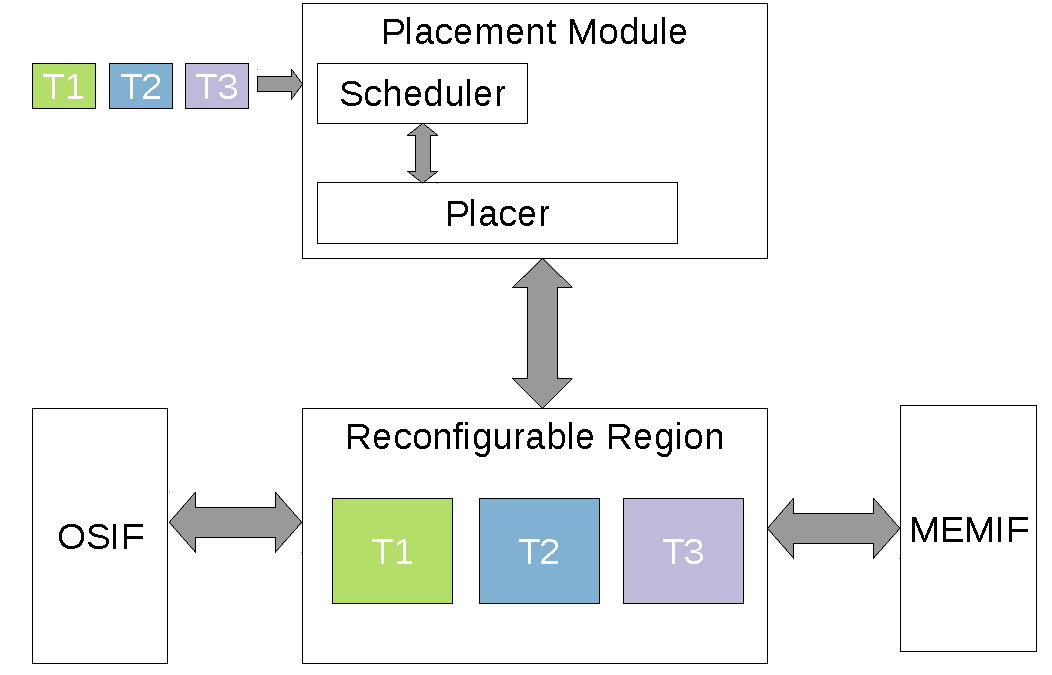
\includegraphics[width=\columnwidth]{graphics/TaskBased.pdf}
    \caption{Task Based Architecture with a memory map for a unified communication interface}\label{fig:TaskBased}
\end{figure}
The placement module is responsible for the determination of a suitable location for a scheduled hardware task based on the \textit{MER-3D Contact algorithm}. 
To achieve this, the \gls{RP} is split into squares of equal size as the smallest possible granularity of logic that may be available to a task.
Hardware tasks contain information about their required width ($T_w$) and height ($T_h$) in relation to the created grid. 
They also contain information about their task arrival time ($T_a$), execution time ($T_e$) and deadline ($T_d$).
Equation \ref{equ:HardwareTask} shows a compact representation of such a hardware task while figure \ref{fig:TaskGrid} shows the subdivided \gls{RP} where the two tasks \textit{T1} and \textit{T2} are already placed and executed.
\begin{equation}\label{equ:HardwareTask}
    HT(T_w, T_h, T_a, T_e, T_d)
\end{equation}
\begin{figure}
    \centering
    %\includegraphics[width=\columnwidth]{}
    \scalebox{0.5}{
    \resizebox{\smallColumnWidth}{!}{\newcommand*{\xMin}{0}%
\newcommand*{\xMax}{3}%
\newcommand*{\yMin}{0}%
\newcommand*{\yMax}{3}%
\newcommand*{\gridScale}{4}
\begin{tikzpicture}
        %\foreach \i in {\xMin,...,\xMax} {
    %    \draw [black] (\i / \gridScale,\yMin / \gridScale) -- (\i / \gridScale,\yMax/ \gridScale);
    %}
    %\foreach \i in {\yMin,...,\yMax} {
    %    \draw [black] (\xMin / \gridScale,\i / \gridScale) -- (\xMax / \gridScale,\i / \gridScale);
    %}

%\draw [step=0.3,blue, very thick] (0.5,0.5) grid (2,2);

\begin{scope}[
    yshift=0,every node/.append style={
        yslant=0,xslant=0},yslant=0,xslant=0
      ]
    %\fill[white,fill opacity=0.6] (0,0) rectangle (5,5);
    \draw[step=10mm, black] (0,0) grid (5,5);
    %\draw[step=2mm, green] (2,2) grid (3,3);
    \fill[cGreen!50, text=black] (0,5) rectangle(2,2) node[pos=0.5] {D1};
    \fill[cBlue!50, text=black] (2,5) rectangle(4,3) node[pos=0.5] {T2};
    \draw[black,very thick] (0,0) rectangle (5,5);
\end{scope}

\end{tikzpicture}}
    }
    \caption{The \gls{RP} is split into a grid to allow the mapping of tasks based on their resource usage}\label{fig:TaskGrid}
\end{figure}
\subsubsection{Fault mitigation scheme}
To mitigate transient and permanent faults, that occur in the \gls{RP} of the \gls{FPGA}, the description of the hardware task is extended with the status of the resource.
If a fault is detected within a square of logic, a new damaged task \textit{D1} is created and bound to the faulty tile (Figure \ref{fig:TaskGridFault}).
It gets the highest priority and the longest possible execution time assigned to prevent other tasks from being placed into the faulty area.
Due to this, the placement algorithm does not need to be modified in any way, as the faulty tile is just treated as a busy task that is reschedule as soon as it expires.
An extension to this would be a new constraint that requires other tasks to be placed as far away from the damaged resource as possible. 
\begin{figure}
    \centering
    %\includegraphics[width=\columnwidth]{}
    \scalebox{0.5}{
    \resizebox{\smallColumnWidth}{!}{\newcommand*{\xMin}{0}%
\newcommand*{\xMax}{3}%
\newcommand*{\yMin}{0}%
\newcommand*{\yMax}{3}%
\newcommand*{\gridScale}{4}
\begin{tikzpicture}
        %\foreach \i in {\xMin,...,\xMax} {
    %    \draw [black] (\i / \gridScale,\yMin / \gridScale) -- (\i / \gridScale,\yMax/ \gridScale);
    %}
    %\foreach \i in {\yMin,...,\yMax} {
    %    \draw [black] (\xMin / \gridScale,\i / \gridScale) -- (\xMax / \gridScale,\i / \gridScale);
    %}

%\draw [step=0.3,blue, very thick] (0.5,0.5) grid (2,2);

\begin{scope}[
    yshift=0,every node/.append style={
        yslant=0,xslant=0},yslant=0,xslant=0
      ]
    %\fill[white,fill opacity=0.6] (0,0) rectangle (5,5);
    \draw[step=10mm, black] (0,0) grid (5,5);
    %\draw[step=2mm, green] (2,2) grid (3,3);
    \fill[cGreen!50, text=black] (0,5) rectangle(2,2) node[pos=0.5] {T1};
    \fill[cRed!50, text=black] (2,5) rectangle(3,3) node[pos=0.5] {D1};
    \fill[cBlue!50, text=black] (3,2) rectangle(5,0) node[pos=0.5] {T2};
    \draw[black,very thick] (0,0) rectangle (5,5);
\end{scope}

\end{tikzpicture}}
    }
    \caption{Damaged task D1 blocks the hardware placer from using the faulty tiles for other tasks}\label{fig:TaskGridFault}
\end{figure}
 
\subsection{Task Based Architecture for \gls{DPR} by Sharma et al.}\label{sec:TaskBasedArchitectureSharma}
The work in \cite{sharma_run-time_2018} proposes a similar architecture to \cite{wang_dynamic_2018} but puts a bigger focus on making adaptions to changes in the available power budget.
That means that \gls{DPR} is utilized to achieve \gls{RT-SA}, i.e. a system that can dynamically alter its architecture to mitigate the effects of changed circumstances.
To achieve this goal, different implementations of the same algorithm need to be provided.
These implementations can differ in the used hardware resources (e.g. area, specific components, routing) to accommodate for different situations.
But as the amount of different implementations increases, it is getting more difficult to choose the optimal combination of modules for a certain setting.
A bigger solution space is especially problematic on a system that already operates on constrained resources, as storage (for a pre-computed look-up table) as well as computational power (for a live exploration) are constrained. 
Therefore, the so called \textit{Explorer} flow is proposed.
This flow allows the selection of a suitable combination of task modules based on the current requirements.
\subsubsection{Fault mitigation scheme}
The \textit{Explorer} also implements a fault mitigation flow.
When a fault is detected in a \gls{RP}, a reconfiguration to another \gls{RP} is attempted as a first step.
If no spare \glspl{RP} are available (i.e. all resources are in usage), it may still be possible to reduce another tasks resource consumption while it stills keeps up the required functionality and meets its deadline.
For this purpose, the task with the lowest priority is examined.
If there is a configuration that fulfils the necessary requirements, the task is reconfigured to this degraded form and the faulty task is moved to the now free spare slot.
Should the lowest priority task already be reduced to its most economical form (in regards to consumed area), the process is repeated with the next higher priority task. 
When the list of possible tasks is exhausted, i.e. the task with the highest priority is reached and no sufficient area could be claimed, another solution needs to be found. 
In this case, the list of of tasks is traversed again from the bottom up. 
This time, each task is checked for a protection flag, the \gls{EC}. 
If this flag is set to 0, the task is eliminated and the faulty task is instantiated in the created spare space.
After a successful mitigation the faulty area is checked for transient and permanent faults. 
In the case of a transient fault, the original configuration is restored after the the faulty tile is recovered. 
For permanent faults, the new configuration is kept and the faulty tile is removed from future evaluation processes. 
 
%\begin{figure}
%    \centering
%    %\includegraphics[width=\columnwidth]{}
%    \scalebox{0.8}{
%    \resizebox{\smallColumnWidth}{!}{% Define block styles
\tikzstyle{decision} = [diamond, draw, fill=blue!20, 
    text width=4.5em, text badly centered, node distance=3cm, inner sep=0pt]
\tikzstyle{block} = [rectangle, draw, fill=blue!20, 
    text width=5em, text centered, rounded corners, minimum height=4em]
\tikzstyle{line} = [draw, -latex']
\tikzstyle{cloud} = [draw, ellipse,fill=red!20, node distance=3cm,
    minimum height=2em]
    
\begin{tikzpicture}[node distance = 3cm, auto]

     %Place nodes
    \node [block] (init) {Hardware Fault Flow};
    \node [block, below of=spareAvailable] (leastPriorityTask) {Select Task with least priority};
    \node [decision, below of=leastPriorityTask] (canReduce) {Can task performance be reduced?};
    \node [block, right of=canReduce] (reducePriority) {Reduce task perfomance};
    \node [block, below of=reducePriority] (findVariant) {Find a more optimal variant};
    \node [decision, below of=canReduce] () {Reduce task perfomance};
    %\node [cloud, left of=init] (expert) {expert};
    %\node [cloud, right of=init] (system) {system};
    %\node [block, below of=init] (identify) {identify candidate models};
    %\node [block, below of=identify] (evaluate) {evaluate candidate models};
    %\node [block, left of=evaluate, node distance=3cm] (update) {update model};
    %\node [decision, below of=evaluate] (decide) {is best candidate better?};
    %\node [block, below of=decide, node distance=3cm] (stop) {stop};
    % Draw edges
    %\path [line] (init) -- (identify);
    %\path [line] (identify) -- (evaluate);
    %\path [line] (evaluate) -- (decide);
    %\path [line] (decide) -| node [near start] {yes} (update);
    %\path [line] (update) |- (identify);
    %\path [line] (decide) -- node {no}(stop);
    %\path [line,dashed] (expert) -- (init);
    %\path [line,dashed] (system) -- (init);
    %\path [line,dashed] (system) |- (evaluate);
\end{tikzpicture}}
%    }
%    \caption{Flow chart for fault mitigation with limited resources}\label{fig:FaultFlowSharma}
%\end{figure}
\section{\gls{DPR} in \glspl{NoC}}\label{sec:NoC}
\glspl{NoC} in \glspl{FPGA} are another example for fault mitigation on the architectural level. 
\glspl{NoC} in general are already designed with fault tolerance in mind, e.g. re-routing packages over different paths to avoid congestion or re-configuration of task mappings to re-balance the network as described in the literature review by \cite{kadri_survey_2019}.
\glspl{NoC} can be seen from two sides in the context of \gls{DPR}. 
Firstly, it can be used as a communication network inside a \gls{RP} (\cite{majer_packet_2005}) and thereby is one way to enable a flexible and heterogeneous task mapping architecture as described in section \ref{sec:TaskBasedArchitectureWang}. 
Secondly, it can be used to link different \glspl{IP} cores together, thereby providing an efficient communication architecture in an otherwise static network.
\cite{wehbe_secure_2016}  introduces a way of not only using \gls{DPR} for the mitigation of transient and permanent faults, but also in the context of security related risks in \glspl{NoC}.
The next two sections will explore these two threat scenarios and present how mitigation can be handled with \gls{DPR}. 

\subsection{Increased security for \gls{DPR}}\label{sec:IncreasedSecurityNoC}
The \gls{NoC} in \cite{wehbe_secure_2016} introduces a security concept that is adapted from the base of public key cryptography. 
They argue that design-time methods alone are not enough to ensure the integrity of all \glspl{IP} that are eligible for \gls{DPR}.
If such a malicious \gls{IP} is instantiated and joins the \gls{NoC} it is able to exploit classic network vulnerabilities (e.g. \gls{DoS} attacks, eavesdropping on traffic, provide malicious data, ...).
Even if a router verifies the authenticity of the node and blocks all future communication from this node, it may still be able to exploit unforeseen security breaches.  

This is, where the public key cryptography comes into play. 
For all \glspl{IP} that are trusted, a public-private key-pair is computed at design time. 
When a node instantiates an \gls{IP} with \gls{DPR}, its authenticity is verified by a security module within the nearest router. 
If that verification fails, the security module triggers a reconfiguration flow that removes all links that connect the malicious \gls{IP} to the rest of the \gls{NoC}.
This reduces the attack vector on the router and thereby assists the prevention of intentionally produced faults. 

\subsection{\gls{DPR} for failed routers}\label{sec:failedRouters}
\glspl{NoC} are also susceptible to transient and permanent faults. 
They are already resilient by design, but especially nodes at the edge of the network (i.e. those that don't have the maximum amount of neighbours) can be cut off from the rest of the network entirely when a fault occurs in the area of their corresponding routers. 
\cite{wehbe_secure_2016} proposes to use \gls{DPR} to change the topology of the network to reconnect the lost node $N_1$ to a healthy router.
For this, a close router $R_1$ is selected. 
The number of network interfaces on each router is constant, so another node $N_x$ needs to be unlinked from router $R_1$. 
This node $N_x$ still needs to be connected to another router $R_n$ after being disconnected from $R_1$, i.e. it needs to remain in the network after the reconfiguration.

Figure \ref{fig:nocSwap} shows a simplified version of the approach taken in \cite{wang_dynamic_2018}. 
Multiple nodes are connected to their respective routers over a \gls{RP}.
It is assumed that \textit{Node 2} is connected to at least two routers, one of which is \textit{Router 2}.
\textit{Node 1} is a corner node that has only a link to one router, namely \textit{Router 1}.
When \textit{Router 1} fails to operate, a reconfiguration process in the \gls{RP} is triggered to reconnect \textit{Node 1} to the rest of the network.
As \textit{Node 2} still has a healthy connection to a second router, it is disconnected from \textit{Router 2} and the free link interface is used for \textit{Node 1}.
\begin{figure}
    \centering
    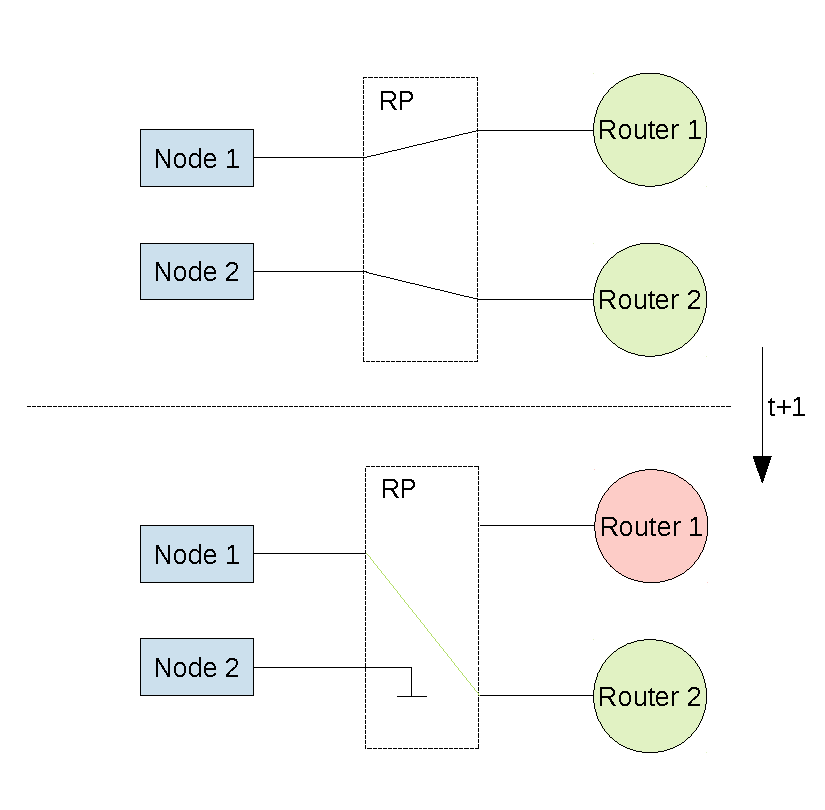
\includegraphics[width=\columnwidth]{graphics/nocSwap.pdf}
    \caption{Simplified process of link reconfiguration, the \gls{RP} is used for switching up the routing.}\label{fig:nocSwap}
\end{figure}
